\documentclass[11pt]{beamer}
% Packages
\usepackage{beamer-german}

% Title etc.
\title{Politisches Wissen und Interesse}
\subtitle{Analyse politischer Unterstützung in der quantitativen Forschungspraxis}
\date{10. Dezember 2021}
\author{B. Philipp Kleer}
\institute{Institut für Politikwissenschaft | Justus-Liebig-Universität Gießen}

\setbeamerfont{itemize/enumerate body}{size = \small}
\setbeamerfont{itemize/enumerate subbody}{size = \footnotesize}
\setbeamerfont{itemize/enumerate subsubbody}{size = \scriptsize}

% Datumspaket
\usepackage[german]{isodate}

% Table packages
\usepackage{booktabs}
\usepackage{longtable}

\addbibresource{lit-s7.bib}

\begin{document}

\begin{frame}
	\maketitle
\end{frame}

\begin{frame}[t]{Präsentationen}
Bitte daran denken, mir bis zum 17. Dezember 2021 eine E-Mail zu schreiben, wenn man die Präsentation in einer Gruppe machen möchte. 

  \begin{itemize}
    \item Ohne Meldung $\Rightarrow$ Einzelpräsentation
    \item Je nach Meldungen werden wir 1 oder 2 Einheiten mit Präsentationen haben
    \item Wichtig: Präsentation ist nicht finaler Projektstand, sondern Arbeitsstand. Offene Fragen sollen benannt und auch in Gruppe dann besprochen werden (Peer-Feedback)
  \end{itemize}
\end{frame}

%\begin{frame}{Textexpert:innen}
%	\begin{itemize}
%		\item \cite{vanDeth2004}:
%		\item \cite{Westle2020}:
%		\item \cite{Reichert2019}:
%		\item \cite{Russo2017}:
%	\end{itemize}
%\end{frame}

\begin{frame}{Zwischenfeedback}
\begin{figure}[ht]
	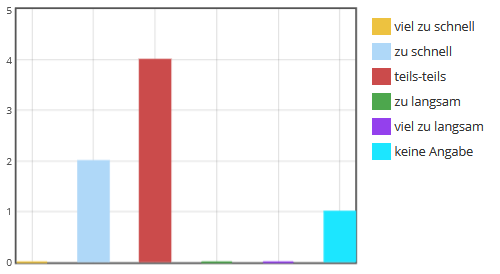
\includegraphics[width=\textwidth]{./pics/lerntempo.png}
	\caption{\textbf{Wähle aus, was auf das Lerntempo deiner Meinung nach im Kurs zutrifft. (n=8)}}
\end{figure}
\end{frame}

\begin{frame}{Zwischenfeedback}
\begin{figure}[ht]
	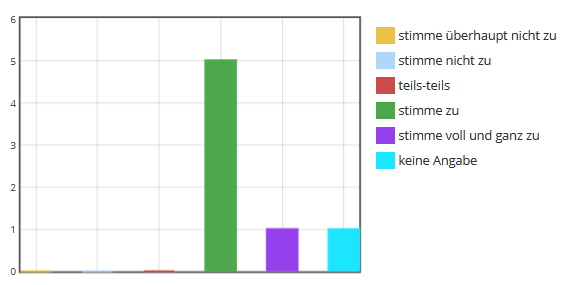
\includegraphics[width=\textwidth]{./pics/lernfortschritt.png}
	\caption{\textbf{Ich erkenne bei mir selbst einen Lernfortschritt. (n=8)}}
\end{figure}
\end{frame}

\begin{frame}{Zwischenfeedback}
\begin{figure}[ht]
	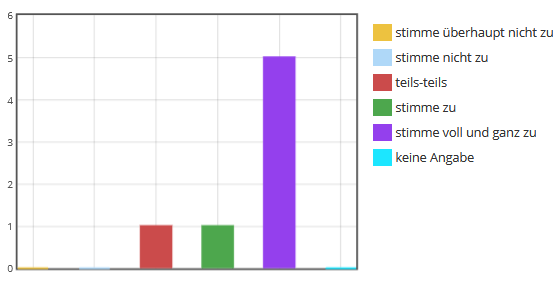
\includegraphics[width=\textwidth]{./pics/wechsel.png}
	\caption{\textbf{Das Verhältnis bzw. der Wechsel zwischen Plenum und Kleingruppe gefällt mir bisher gut. (n=8)}}
\end{figure}
\end{frame}

\begin{frame}{Zwischenfeedback: Freitext-Antworten}
\scriptsize
\begin{itemize}
	\item Bisher noch keine Anmerkungen, das Tempo und der Inhalt korrelieren gut miteinander
	\item Die Ideen sind sehr gut, leider konnte ich noch nicht viel vom Seminar sehen.
	\item Sehr interessant und lehrreich bis jetzt.
	 \item Aufgrund des Umfangs der Literatur und der komplizierten Theorien, die in jeder Sitzung gelesen werden müssen, hoffe ich, die wichtigsten Leitfragen, die im Unterricht gelöst werden müssen, im Voraus zu geben.
	 \item Mir gefällt das Seminar auf jeden Fall sehr gut, jedoch bereiten mir die englischen Lektüren häufig ein Problem und rauben mir dadurch viel Zeit und Kraft bis ich sie weitestgehend verstanden habe. Natürlich wäre es wünschenswert, wenn wir nur auf deutsche Texte zurückgreifen könnten, jedoch kann ich gut nachvollziehen, dass wir uns auch mit englischer sprachiger Literatur auseinandersetzen müssen. Ebenfalls wollte ich anmerken, dass ich die Lernatmosphäre sehr schätze. Es gibt bei dir im Seminar keine Hemmschwelle wie in anderen Onlineseminaren, die mich davon abhält mich zu beteiligen.
	 \item Ehrlich gesagt bin ich nicht so gut in SPSS wie ich es vielleicht sein sollte. Das kann daran liegen, dass ich teilweise Sachen vergessen habe oder das ich weniger mitgenommen habe wegen der Online Lehre, die ich mir generell manchmal schwerer fällt. deshalb komme ich nicht so wirklich mit, wenn wir SPPS Übungen machen.
\end{itemize}
\end{frame}

%\begin{frame}[t]{Triggerwarnung}
%Ihr habt einen Trigger erwischt, daher jetzt die \shine{Dozentenantwort}:
%
%  \begin{itemize}
%    \item Sozialwissenschaften ist eine Buch-Wissenschaft!
%    \item Lese-Umfang für Gießen evtl. hoch
%    \item[$\Rightarrow$] im Vergleich mit anderen Universitäten normaler Pflichtlektüre-Umfang (i.d.R. 50-100 Seiten pro Veranstaltung pro Woche)
%  \end{itemize}
%\end{frame}

\begin{frame}{Aufgabe}
Tauscht euch in der Kleingruppe kurz über die grundlegenden Defintiionen des Textes aus. 

Diskutiert auch die zwei Fragen aus dem Etherpad:
\begin{nolist}
	\item Was genau meint der Autor mit Salienz? $\Rightarrow$ Ein Thema ist präsenter/ wichtiger d.h. salienter?
	\item Beschränkt sich kognitives politisches Engagement essentiell auf Nachdenken über Politik? Oder kann man den Begriff eher als Verstehen von Politik definieren? Ist das Internet als Informationsquelle für nationale und europäische Nachrichten wirklich so unwichtig wie aus den Daten von Westle hervorgeht?
\end{nolist}

\shine{Zeit: 15 Min.}
 
\end{frame}

\section{Definitionen}

\setbeamerfont{itemize/enumerate body}{size = \scriptsize}

\begin{frame}[t]{Politisches Interesse}
			\shine{Political Interest} \pause
			\begin{itemize}
				\item “degree to which politics arouses a citizen’s curiosity” \parencite[278]{vanDeth1990}
				\item “citizen’s willingness to pay attention to political phenomena at the possible expense of other topics” \parencite[1122]{Lupia2005}
				\item "the extent to which an individual pays attention to politics" \parencite[21]{Zaller1992} \pause
				\item[$\Rightarrow$] Konzeptuell: Grad der Aufmerksamkeit, Häufigkeit politischer Diskussionen, persönliche Bedeutung von Politik, Salienz von Politik
			\end{itemize}
		\end{frame}

\setbeamerfont{itemize/enumerate body}{size = \scriptsize}

\begin{frame}[t]{Politisches Interesse}
			\shine{Kognitives politisches Engagement} \pause
			\begin{itemize}
				\item habituelle Aufmerksamkeit gegenüber Politik, Fakten-kenntnisse und Verständnis politischer Vorgänge und Normen im Zentrum \parencite{Zaller1992}
				\item „generelle Interesse an Politik, die Bereitschaft zur Teilhabe am politischen System und die Evaluation der Möglichkeit einer entsprechenden Teilhabe“ \parencite[72]{Pickel2002}
				\item allgemeines Politikinteresse und in weiterem Sinn das „Ausmaß der individuellen psychologischen Verbundenheit mit dem politischen System“ \parencite[72f]{Caballero2009}
				\item Interesse und Wichtigkeit von Politik \parencite{Martin2007}
			\end{itemize}
\end{frame}

\setbeamerfont{itemize/enumerate body}{size = \small}

\begin{frame}{Politisches Wissen}
\shine{Politisches Wissen} \pause
	\begin{itemize}
		\item “the range of factual information about politics that is stored in long-term memory” \parencite[10]{DelliCarpini1996}
		\item „currency of citizenship“, which citizens need to be engaged in political decisions \parencite[8]{DelliCarpini1996}
	\end{itemize}
\end{frame}

\section{Was beeinflusst polit. Interesse?}

\begin{frame}{Determinanten polit. Interesse \parencite{vanDeth2004}}
	\begin{itemize}
		\pause
		\item	Niveau politisches Interesse: soziodemographische Faktoren (Schuldbilung, Einkommen, gesellschaftliche Position)
		\item Bildung: $\uparrow$ kognitive Aspekte \& Niveau von politischem Interesse, $\uparrow$ Bedeutung von Politik positiv
		\item Einkommen: $\downarrow$ Salienz von Politik
		\item Soziale Kontakte: Mitgliedschaften in Vereinen und Verbänden, Vermeidung politischer Themen möglich, aber auch gegensätzlich möglich
		\item Zufriedenheit: $\uparrow$ Engagement \& politisches Interesse, aber auch $\downarrow$ Bedeutung von Politik und Salienz von Politik
		\item Vertrauen: gering $\rightarrow$ $\downarrow$ Politisches Interesse, relevant für Niveau politisches Interesse und Häufigkeit politischer Gespräche
	\end{itemize}
\end{frame}

\begin{frame}{Kognitives Politisches Engagement \parencite{Westle2020}}
	\begin{itemize}
		\item	„Als Voraussetzung dafür sollten die Bürger sich für Politik interessieren, ihr kontinuierlich Aufmerksamkeit schenken, und so politisches Wissen und Verständnis sowie Selbstbewusstsein und Handlungskompetenzen als politische Akteure erwerben” \parencite[273]{Westle2020}
	\end{itemize}
	
	\shine{Eigenschaften:} \pause
	\begin{itemize}
		\item Engagement = Beschäftigung \parencite[278]{Westle2020}
		\item Begrenzung auf das Politische \parencite[278]{Westle2020}
		\item Kognitive Prägung ist zentral (nicht affektiv, motivational, evaluativ, konativ oder behavioral \parencite[278]{Westle2020} \pause
		\item[$\Rightarrow$] Nicht vermischen mit Konzepten politischer Unterstützung (z.B. externale Dimension von politischer Effektivität)
	\end{itemize}
\end{frame}

\begin{frame}{Kognitives Politisches Engagement \parencite{Westle2020}}
\shine{Vorschlag an Dimensionen}
	\begin{nolist}
		\item Interesse an und Wichtigkeit von Politik
		\item Informationsverhalten
		\item Bereitschaft zu Diskussion
		\item Faktenwissen
		\item Verständnis von Politik in Form der ideologischen Konzeptualisierungsfähigkeit/Einstellungskonsistenz (Effektivität)
	\end{nolist}
\end{frame}

\renewcommand*{\bibfont}{\scriptsize}

\begin{frame}{Aufgabe}
\shine{GLES-Datensatz: Vorwahlstudie 2017}

	\begin{nolist}
		\item Finde Variablen zum Politischen Wissen. 
		\item Bilde über diese Variablen einen Summenindex. Überlege, wie du den Summenindex bildest und beachte die gelernten Rekodierungsschritte.
	\end{nolist}

\shine{Zeit:} 20-30 Minuten.
\end{frame}

\section{Mittagspause! \\ Wir treffen uns um 12:30 Uhr wieder.}

\begin{frame}[allowframebreaks]{Literatur}
	\nocite{*}
	\printbibliography[heading = none]
\end{frame}

\end{document}
